\section*{\textcolor{orange}{سوال 1:}}
پیاده‌‌سازی یک روش نهان‌کاوی به عنوان آشکارسازی بر نهان‌نگاری به روش \lr{LSB} .یعنی فرض کنید که ما با روش \lr{LSB} عملیات نهان‌نگاری را انجام دادیم، شما باید یک روش نهان‌کاوی به منظور تشخیص آن پیاده‌سازی کنید.
\subsection*{\textcolor{cyan}{پاسخ 1:}}
کد موردنظر برای این بخش را در فایل \lr{Q1.ipynb} پیاده‌سازی کردیم. برای اینکه یک تصویر داشته باشیم تا بتوانیم عملیات نهان‌کاوی را روی آن انجام دهیم، در کدمان یک بخش برای \lr{encode} کردن تصویر، و یک بخش برای \lr{decode} آن قرار دادیم. سپس تصویر موردنظر را با پیام دلخواه \lr{encode} کردیم. همانطور که می‌دانیم در این روش برای \lr{encode} کردن تصویر، پیام در بیت‌های \lr{LSB} پیکسل‌ها قرار می‌گیرند؛ چرا که این بیت‌ها کم‌ارزش‌ترین بیت‌ها هستند و تغییر در آن‌ها، تفاوت چندانی در تصویر ایجاد نمی‌کند. در تابع \lr{Encode}، این اتفاق می‌افتد.
\begin{figure}[H]
  \centering
  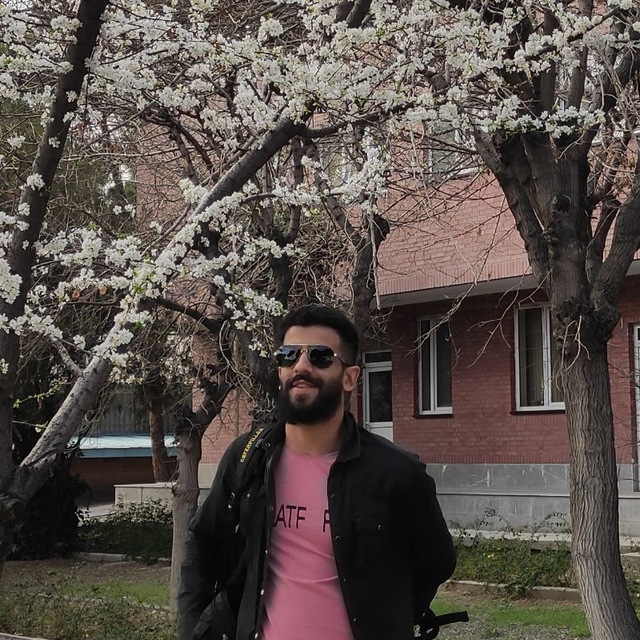
\includegraphics[width=0.65\textwidth]{Images/farzan.png}
  \caption{تصویر اصلی قبل از عملیات \lr{encoding}}   
\end{figure}
حال پس از انتخاب تصویر موردنظر برای عملیات نهان‌کاوی، برنامه را \lr{run} کرده و گزینه \lr{encode} را انتخاب می‌کنیم تا تصویر رمزگذاری شده برای مرحله بعد را آماده نماییم. همچنین کلمه \lr{Security} را به عنوان پیام پنهان به برنامه می‌دهیم. در انتها نیز آدرس مقصد برای ذخیره عکس \lr{encode} شده را می‌دهیم.
\begin{figure}[H]
  \centering
  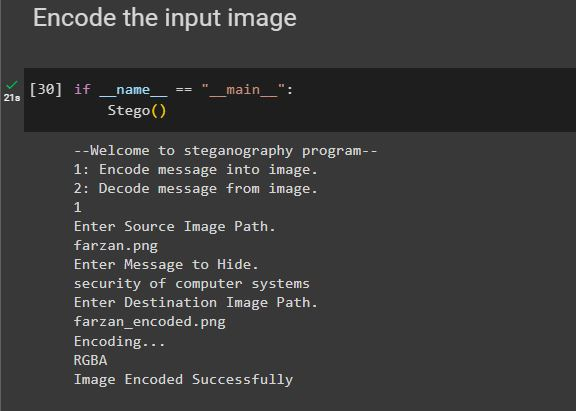
\includegraphics[width=0.7\textwidth]{Images/q1_1.JPG}
  \caption{نحوه \lr{encode} کردن تصویر}   
\end{figure}
حال تصویر رمزنگاری شده را بررسی می‌کنیم. همانطور که در شکل زیر نیز می‌بینید، تصویر رمزنگاری شده تفاوت چندانی با تصویر اصلی ندارد؛ به‌گونه‌ای که تغییرات با چشم غیرمسلح قابل مشاهده نیست. یکی از دلایل این پدیده می‌تواند کوتاه بودن متن پیام باشد. عبارت \lr{\$t3g0} به کار رفته هنگام ذخیره‌سازی تصویر نیز برای تشخیص انتهای پیام می‌باشد.
\begin{figure}[H]
  \centering
  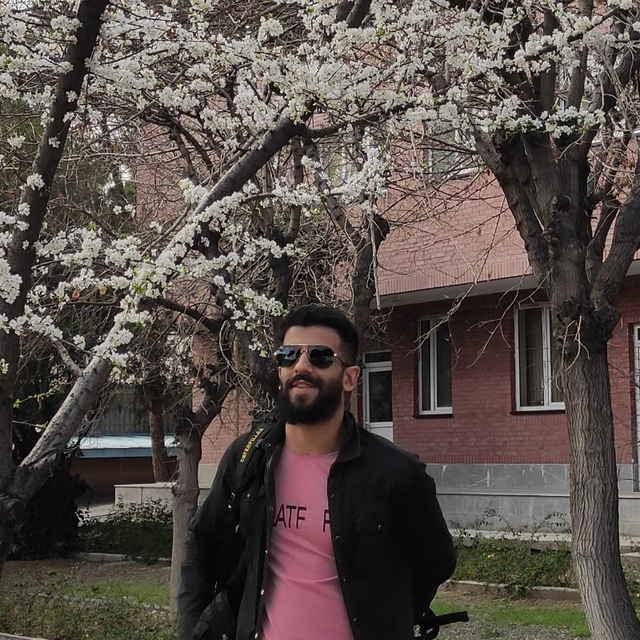
\includegraphics[width=0.5\textwidth]{Images/farzan_encoded.png}
  \caption{تصویر \lr{encode} شده}   
\end{figure}
حال از تابع \lr{Decode} برای نهان‌کاوی تصویر \lr{encode} شده استفاده می‌نماییم. همانطور که در شکل زیر مشاهده می‌نمایید، برنامه به‌درستی کلمه \lr{Security} که به عنوان پیام پنهان به تابع \lr{Encode} داده بودیم را برای ما چاپ می‌کند.
\begin{figure}[H]
  \centering
  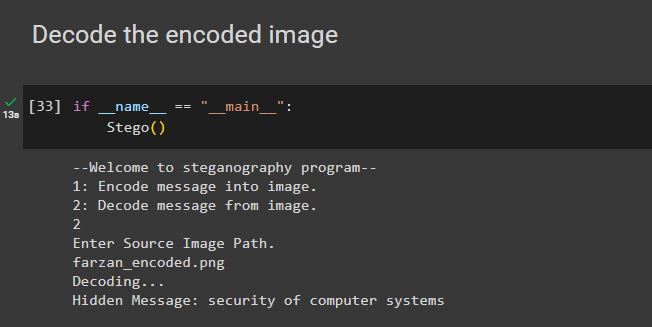
\includegraphics[width=0.6\textwidth]{Images/q1_2.JPG}
  \caption{نحوه \lr{decode} کردن تصویر}   
\end{figure}
\begin{latin}
\href{https://medium.com/swlh/lsb-image-steganography-using-python-2bbbee2c69a2}{\textcolor{blue}{Reference}}
\end{latin}